\documentclass[tikz,border=5pt]{standalone}
\usepackage{amsmath}
\usetikzlibrary{positioning, arrows}

\begin{document}
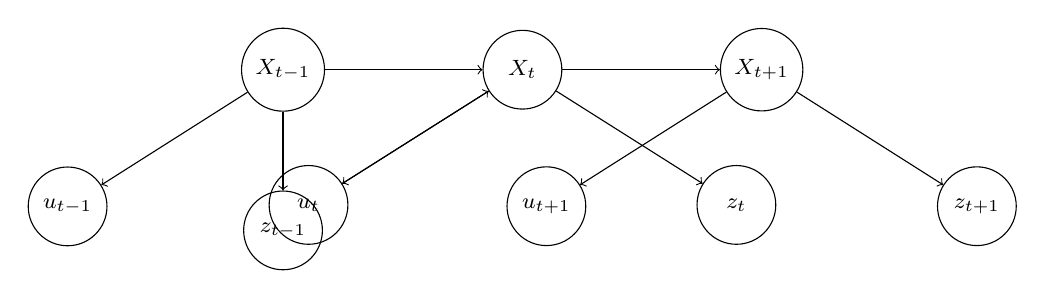
\begin{tikzpicture}[
        node distance=1cm and 2cm,
        every node/.style={circle, draw, minimum size=1cm, font=\footnotesize, align=center},
        every edge/.style={draw, ->, >=stealth}
    ]

    % Nodes at time t-1
    \node (xt-1) {$X_{t-1}$};
    \node[below left=of xt-1] (ut-1) {$u_{t-1}$};
    \node[below=of xt-1] (zt-1) {$z_{t-1}$};

    % Nodes at time t
    \node[right=of xt-1] (xt) {$X_t$};
    \node[below left=of xt] (ut) {$u_t$};
    \node[below right=of xt] (zt) {$z_t$};

    % Nodes at time t+1
    \node[right=of xt] (xt+1) {$X_{t+1}$};
    \node[below left=of xt+1] (ut+1) {$u_{t+1}$};
    \node[below right=of xt+1] (zt+1) {$z_{t+1}$};

    % Edges time t-1 to t
    \draw[->] (xt-1) -- (xt);
    \draw[->] (xt-1) -- (ut-1);
    \draw[->] (xt-1) -- (zt-1);

    % Edges time t to t+1
    \draw[->] (xt) -- (xt+1);
    \draw[->] (xt) -- (ut);
    \draw[->] (xt) -- (zt);
    \draw[->] (ut) -- (xt);

    % Edges time t+1
    \draw[->] (xt+1) -- (ut+1);
    \draw[->] (xt+1) -- (zt+1);

\end{tikzpicture}
\end{document}
